\section{Experiments}


% \textbf{Inference details}. In the inference stage, we employ the DDIM~\cite{song2020denoising} sampler with 50 steps, classifier-free guidance of magnitude 7.0 during inference. \ly{todo: how to conduct cfg on text prompts?}

We conduct experiments on five tasks, including camera control, motion transfer, mesh-to-video generation, and object manipulation to demonstrate the versatility of \methodname in controlling the video generation process. 



% \begin{table}[]
% \centering
% \begin{tabular}{ccccc}
% \hline
% Method        & PSNR $\uparrow$ & SSIM $\uparrow$ & LPIPS $\downarrow$ & FVD $\downarrow$ \\ \hline
% CogVideoXFun  & 9.62            & 0.316           & 0.667              & 1650.3           \\
% CogVideoX-Depth & 18.08           & 0.573           & 0.312              & 645.1            \\
% Ours          & \textbf{19.27}  & \textbf{0.658}  & \textbf{0.261}     & \textbf{551.3}   \\ \hline
% \end{tabular}
% \caption{Quantitative Evaluations. We evaluate the appearance (PSNR, SSIM, LPIPS, FVD) of generated videos on the validation set of the DAVIS and MiraData datasets. The baseline model is trained within depth estimation conditions.}
% \label{tab:i2v}
% \end{table}


\subsection{Camera control}

\textbf{Baseline methods}. To evaluate the ability to control camera motions of generated videos, we select two representative methodologies, MotionCtrl~\cite{wang2024motionctrl} and CameraCtrl~\cite{he2024cameractrl} as baseline methods, both of which allow camera trajectories as input and use camera or ray embeddings for camera control.

\noindent\textbf{Metrics}. To measure the accuracy of the camera trajectories of generated videos, we evaluate the consistency between the estimated camera poses from the generated videos and the input ground-truth camera poses using rotation errors and translation errors.
Specifically, for each frame of a generated video, we reconstruct its relative pose given the first frame using SIFT~\cite{ng2003sift}. Then, we get the normalized quaternion and translation vectors for the rotation and translation. Finally, we calculate the cosine similarity between the estimated camera poses with the given camera poses.
\[
\mathbf{RotErr} = \arccos\left(\frac{1}{T-1} \sum_{i=2}^{T} \langle \;\mathbf{q}_{\mathrm{gen}}^i , \mathbf{q}_{\mathrm{gt}}^i \;\rangle\right),
\]
\[
\mathbf{TransErr} = \arccos \left(\frac{1}{T-1} \sum_{i=2}^{T} \langle\; \mathbf{t}_{\mathrm{gen}}^i , \mathbf{t}_{\mathrm{gt}}^i \;\rangle\right),
\]
where $T$ is the number of frames, $\mathbf{q}^{i}$ and $\mathbf{t}^{i}$ are the normalized quaternion and translation vector of the $i$-th frame, and $\langle \cdot, \cdot \rangle$ means the dot product between two vectors.



\noindent\textbf{Results}.
We compare against baseline methods on 100 random trajectories from RealEstate10K~\cite{zhou2018stereo}. But since most of the random trajectories only contain small movements, we further test the models on larger fixed movements (moving left, right, up, down, spiral) as shown in Figure~\ref{fig:camctrl}. As shown in Table~\ref{tab:camctrl}, our method outperforms the baseline methods, which demonstrates that our method achieves stable and accurate control of the camera poses of the generated videos. The main reason is that due to the utilization of the 3D tracking videos, our method is fully 3D-aware to enable accurate spatial inference in the video generation process. In comparison, baseline methods~\cite{he2024cameractrl,wang2024motionctrl} only adopt implicit camera or ray embeddings for camera control.


\begin{table}[]
\begin{tabular}{cllll}
\hline
Method     & \multicolumn{2}{c}{\textbf{Small Movement}} & \multicolumn{2}{c}{\textbf{Large Movement}} \\
           & TransErr $\downarrow$             & RotErr    $\downarrow$            & TransErr      $\downarrow$         & RotErr     $\downarrow$           \\ \hline
MotionCtrl & 44.23                  & 8.92                  & 67.05          & 39.86                  \\
CameraCtrl & 42.31                  & 7.82                  & 66.76                   & 29.70                 \\
Ours       & \textbf{27.85}         & \textbf{5.97}         & \textbf{37.17}                  & \textbf{10.40}         \\ \hline

\end{tabular}
\caption{\textbf{Quantitative results on camera control} of MotionCtrl~\cite{wang2024motionctrl}, CameraCtrl~\cite{he2024cameractrl}, and our method. ``TransErr'' and ``RotErr" are the angle differences between the estimated translation and rotation and the ground-truth ones in degree.}
\label{tab:camctrl}
\end{table}

\begin{figure*}[htbp]
    \centering
    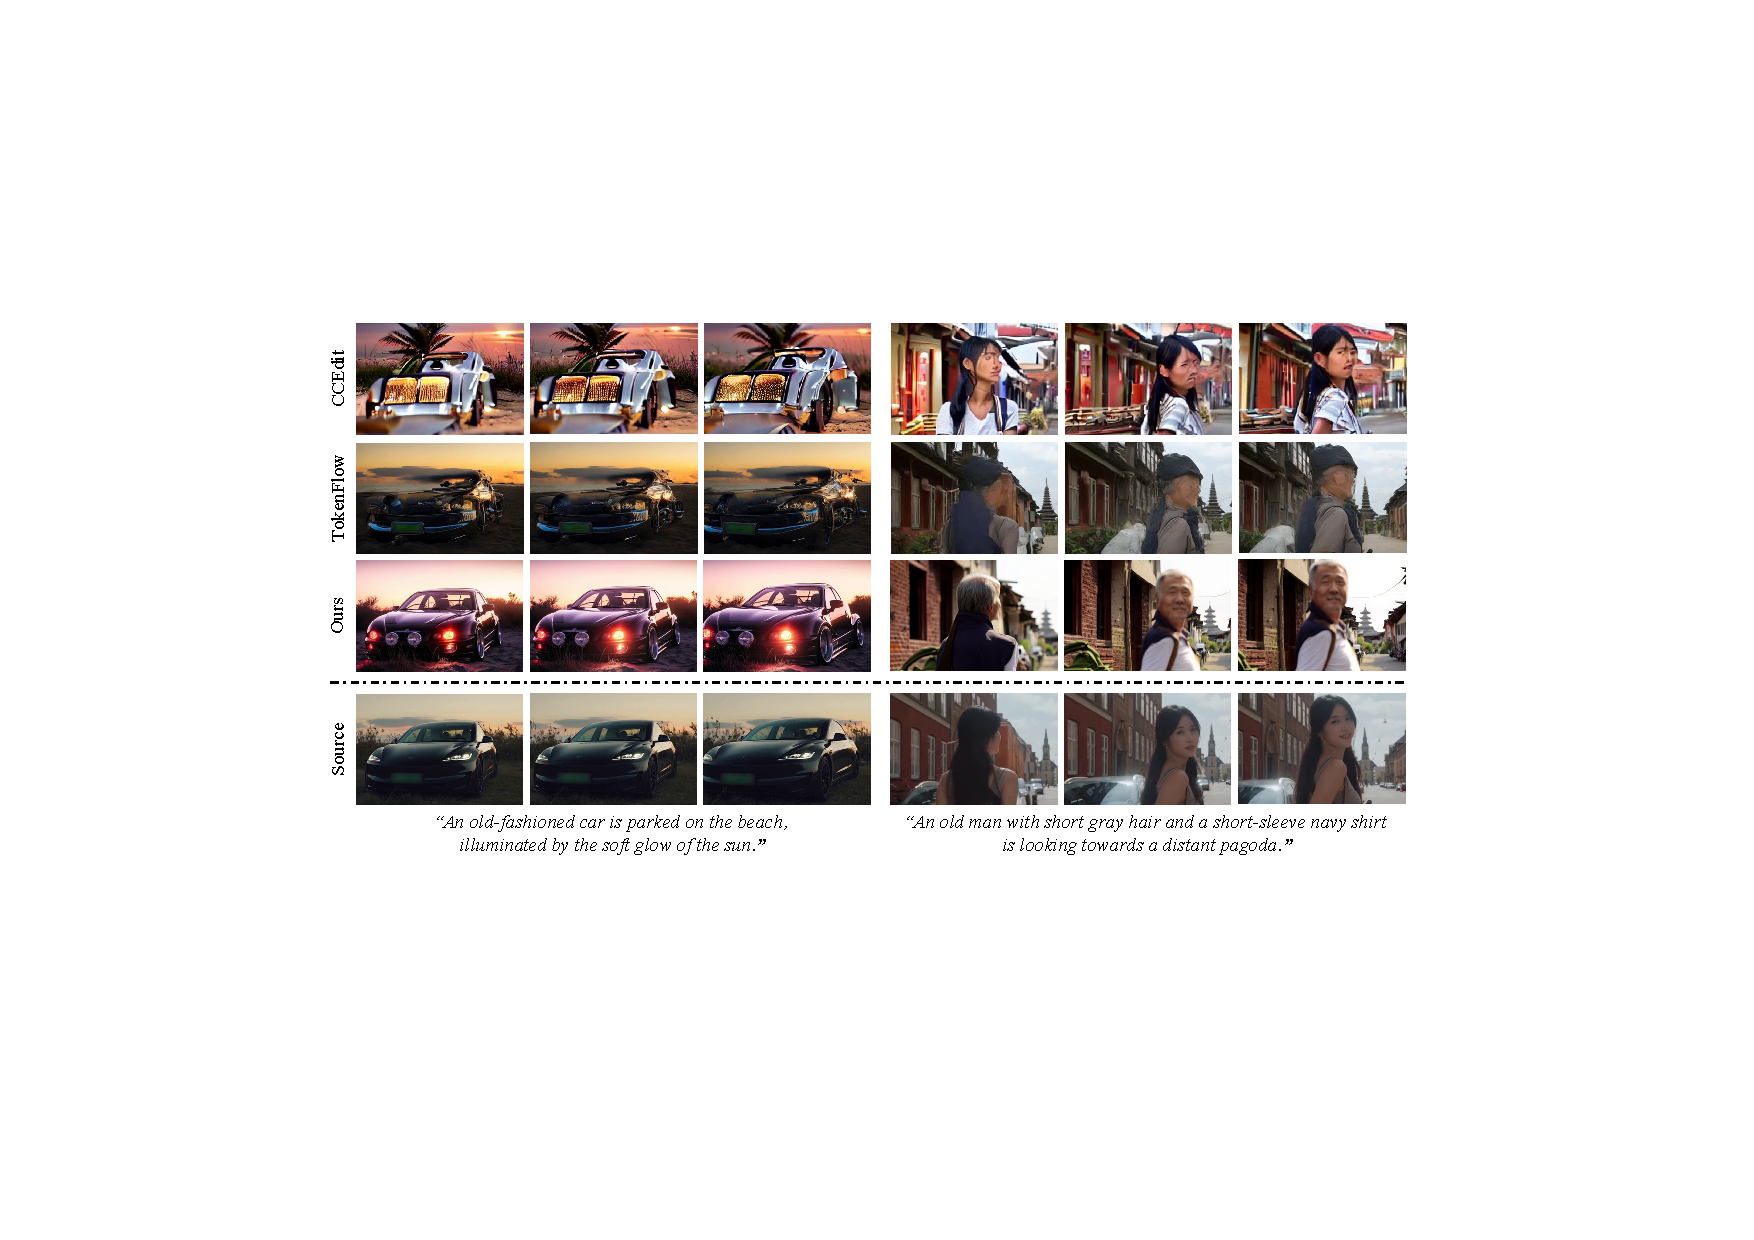
\includegraphics[width=\textwidth]{pictures/v2v2.pdf}
    \caption{\textbf{Qualitative comparison on motion transfer} between our method, CCEdit~\cite{ccedit}, and TokenFlow~\cite{tokenflow}.}
    \label{fig:v2v2}
\end{figure*}

\subsection{Motion transfer}

% \begin{figure}
%     \centering
%     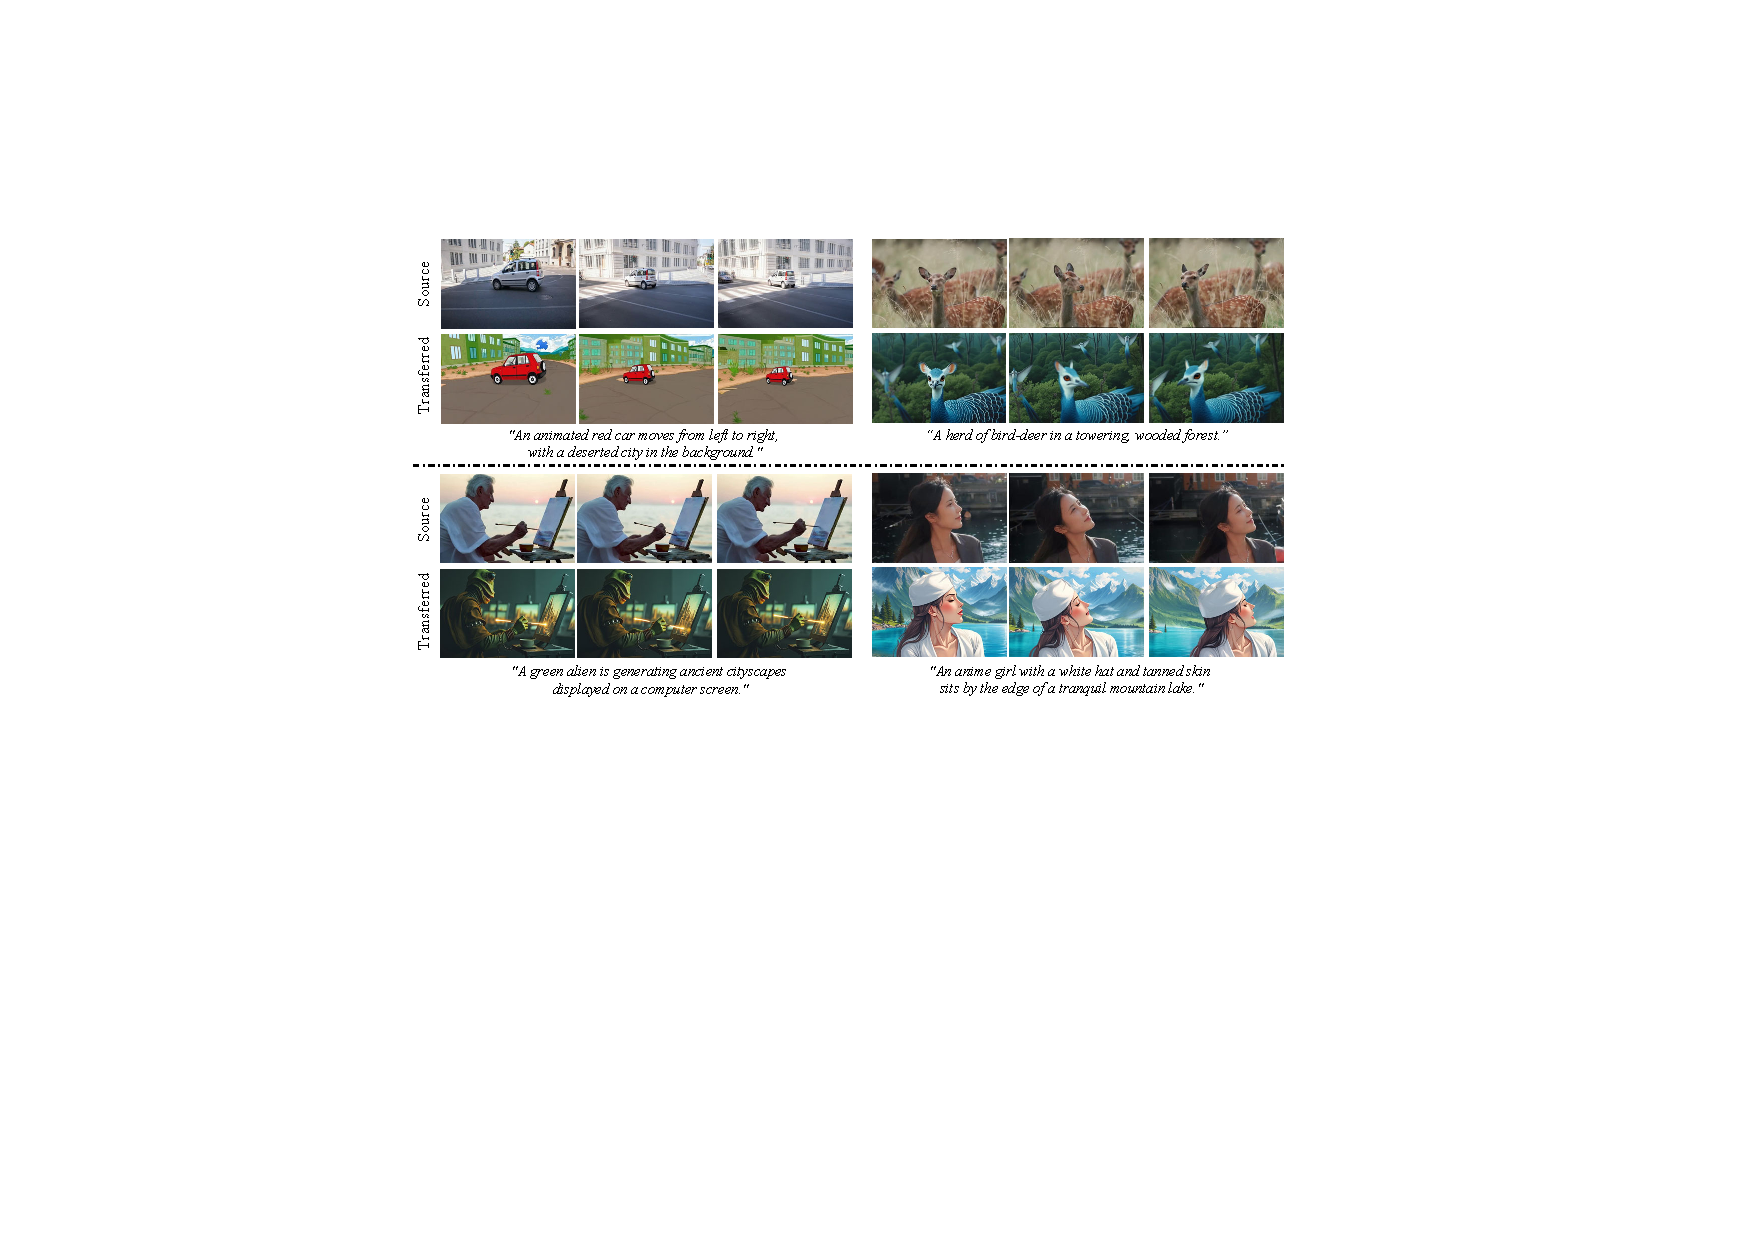
\includegraphics[width=\linewidth]{pictures/v2v1.pdf}
%     \caption{Motion retargeting}
%     \label{fig:v2v1}
% \end{figure}


\noindent\textbf{Baseline methods}. We compare \methodname with two famous motion transfer methods, TokenFlow~\cite{tokenflow} and CCEdit~\cite{ccedit}. TokenFlow represents video motions with the feature consistency across different timesteps extracted by a diffusion model. Then, the feature consistency is propagated to several keyframes generated by a text prompt for video generation. For TokenFlow, we adopt the Stable Diffusion 2.1~\cite{rombach2022high} model for the motion transfer task. CCEdit adopts depth maps as conditions to control the video motion and transfers the motion using a new repainted frame to generate a video. 
% To ensure fairness in comparison, Stable Diffusion-v2.1 is used as the base model for all methods. 

\noindent\textbf{Metrics}. 
Since all methods generate the transferred videos based on text prompts, we aim to evaluate the alignment between the generated videos and the text prompts, as well as the video coherence, using the CLIP \cite{radford2021learningtransferablevisualmodels}. Specifically, for video-text alignment, we extract multiple frames from the video and compare them with the corresponding text prompts by calculating the CLIP score \cite{hessel2022clipscorereferencefreeevaluationmetric} for each frame. This score reflects the alignment between image content and textual descriptions. For temporal consistency, we extract normalized CLIP features from adjacent video frames and compute the cosine similarity between the adjacent features. 

\noindent\textbf{Results}. As shown in Table~\ref{tab:motion}, our method demonstrates outstanding performance in both text alignment and frame consistency, surpassing two baseline methods. Furthermore, \autoref{fig:v2v2} presents the qualitative comparison of our method, CCEdit, and TokenFlow. It shows that CCEdit produces frames of low quality and struggles to maintain temporal coherence. TokenFlow produces semantically consistent frames but has difficulty producing coherent videos. In contrast, our method accurately transfers the video motion with strong temporal coherence as shown in Figure~\ref{fig:v2v1}. 

\begin{table}[]
\centering
\begin{tabular}{lcc}
\hline
Method                           & \multicolumn{1}{c}{Tex-Ali} $\uparrow$ & \multicolumn{1}{c}{Tem-Con} $\uparrow$ \\ \hline
CCEdit                           & 16.9& 0.932 \\
Tokenflow                        & 31.9& 0.956 \\
Ours                             & \textbf{32.6}& \textbf{0.971} \\
\hline
\end{tabular}
\caption{\textbf{CLIP scores for motion transfer} of CCEdit~\cite{ccedit}, TokenFlow~\cite{tokenflow}, and our method. ``Text-Ali'' is the semantic CLIP consistency between generated videos and the given text prompts. ``Tem-Con'' is the temporal CLIP consistency between neighboring frames.}
\vspace{-15pt}
\label{tab:motion}
\end{table}


\begin{figure*}[htbp]
    \centering
    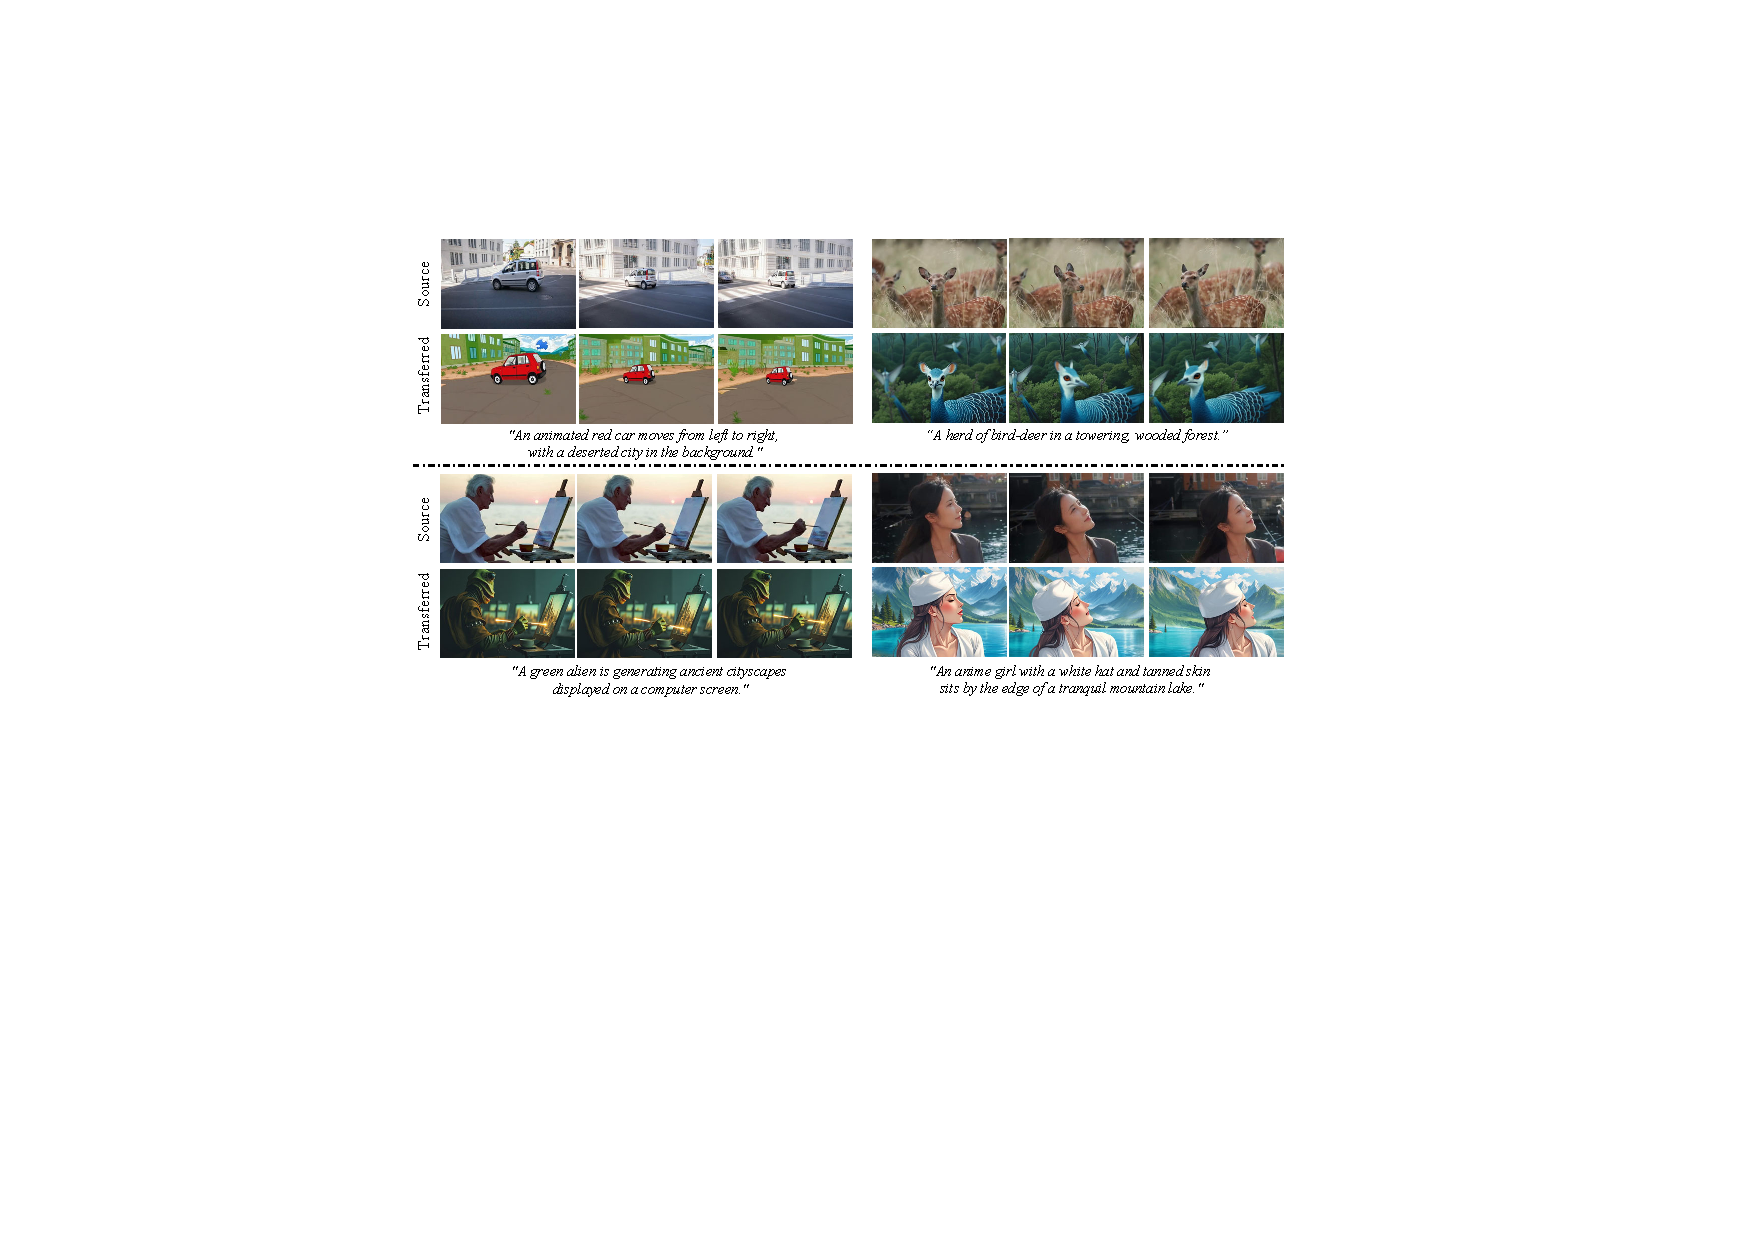
\includegraphics[width=\textwidth]{pictures/v2v1.pdf}
    \caption{\textbf{Qualitative results on motion transfer of our method}.}
    \label{fig:v2v1}
\end{figure*}

\subsection{Animating meshes to videos}
\textbf{Qualitative comparison}. We compare our method against a state-of-the-art human image animation method CHAMP \cite{zhu2024champ} on the mesh-to-video task. 
Champ takes a human image and a motion sequence as input and generates a corresponding human video. The motion sequence is represented by an animated SMPL~\cite{loper2023smpl} mesh. We use the same input image but the SMPL mesh for CHAMP and generate the corresponding animation videos for qualitative comparison as shown in \autoref{fig:m2v2}. We also generate different styles of videos from the same animated 3D meshes as shown in \autoref{fig:m2v2}.
% Champ leverages the 3D human mesh model to establish a unified representation of body shape and pose. Using the same mesh model, we generate corresponding 3D tracking videos, depth maps, skeletons, and semantic representations as inputs for both our model and CHAMP. Additionally, we use FLUX~\cite{flux} to stylize the first-frame reference human image, enabling the models to generate animations.
% The qualitative comparison results are shown in \autoref{fig:m2v2}.
% a comparative analysis is conducted between our approach and CHAMP for cross-identity animation, specifically focusing on animating reference images with videos of different motion sequences and reference images of varying styles. 
Compared to CHAMP, our method demonstrates better consistency in the 3D structure and texture details of the avatar on different motion sequences and across different styles. 
% \autoref{fig:m2v1} presents additional evaluation results of cross-identity animation, including different styles, meshes, and motions.

\begin{figure*}
    \centering
    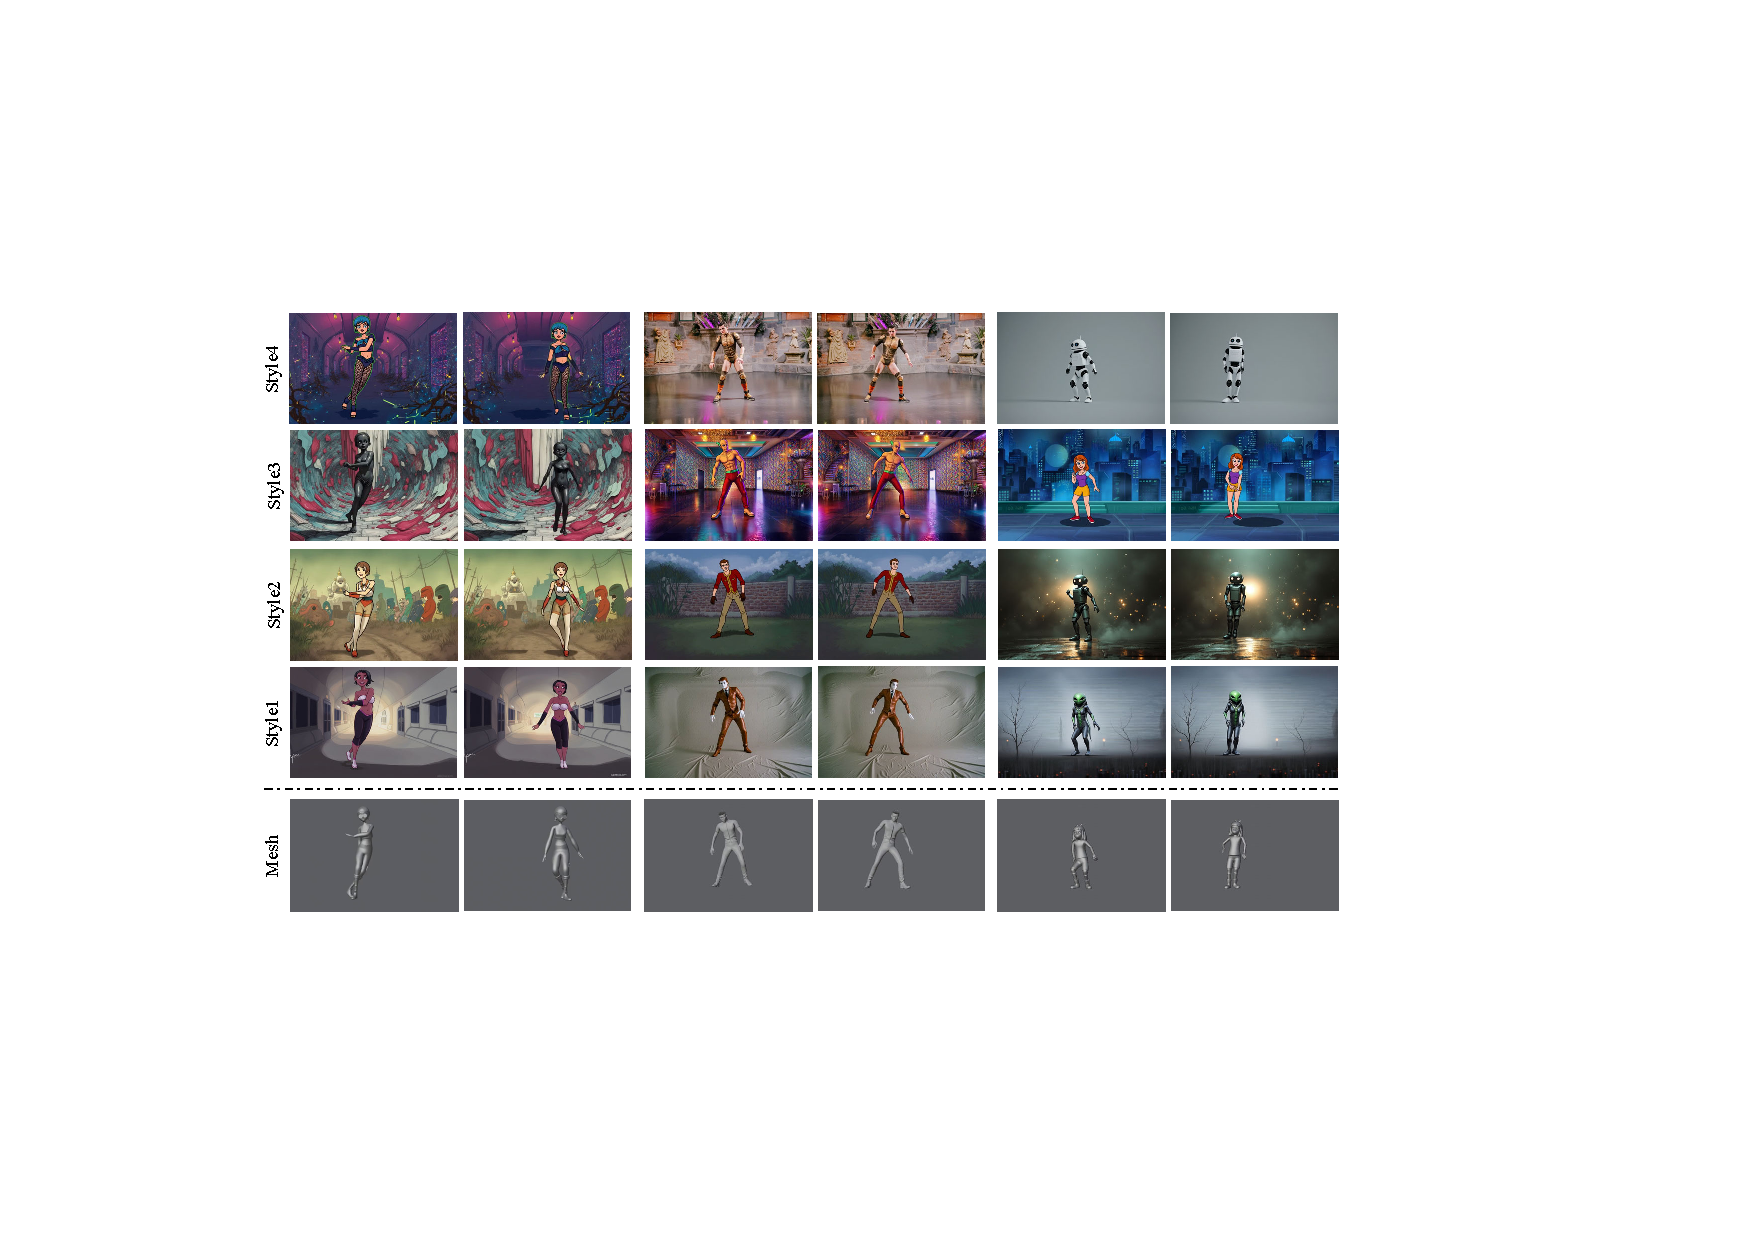
\includegraphics[width=\textwidth]{pictures/m2v1.pdf}
    \caption{\textbf{More results of the animating mesh to video generation task}. Our method enables the generation of different styles from the same mesh.}
    \label{fig:m2v1}
\end{figure*}

\begin{figure*}
    \centering
    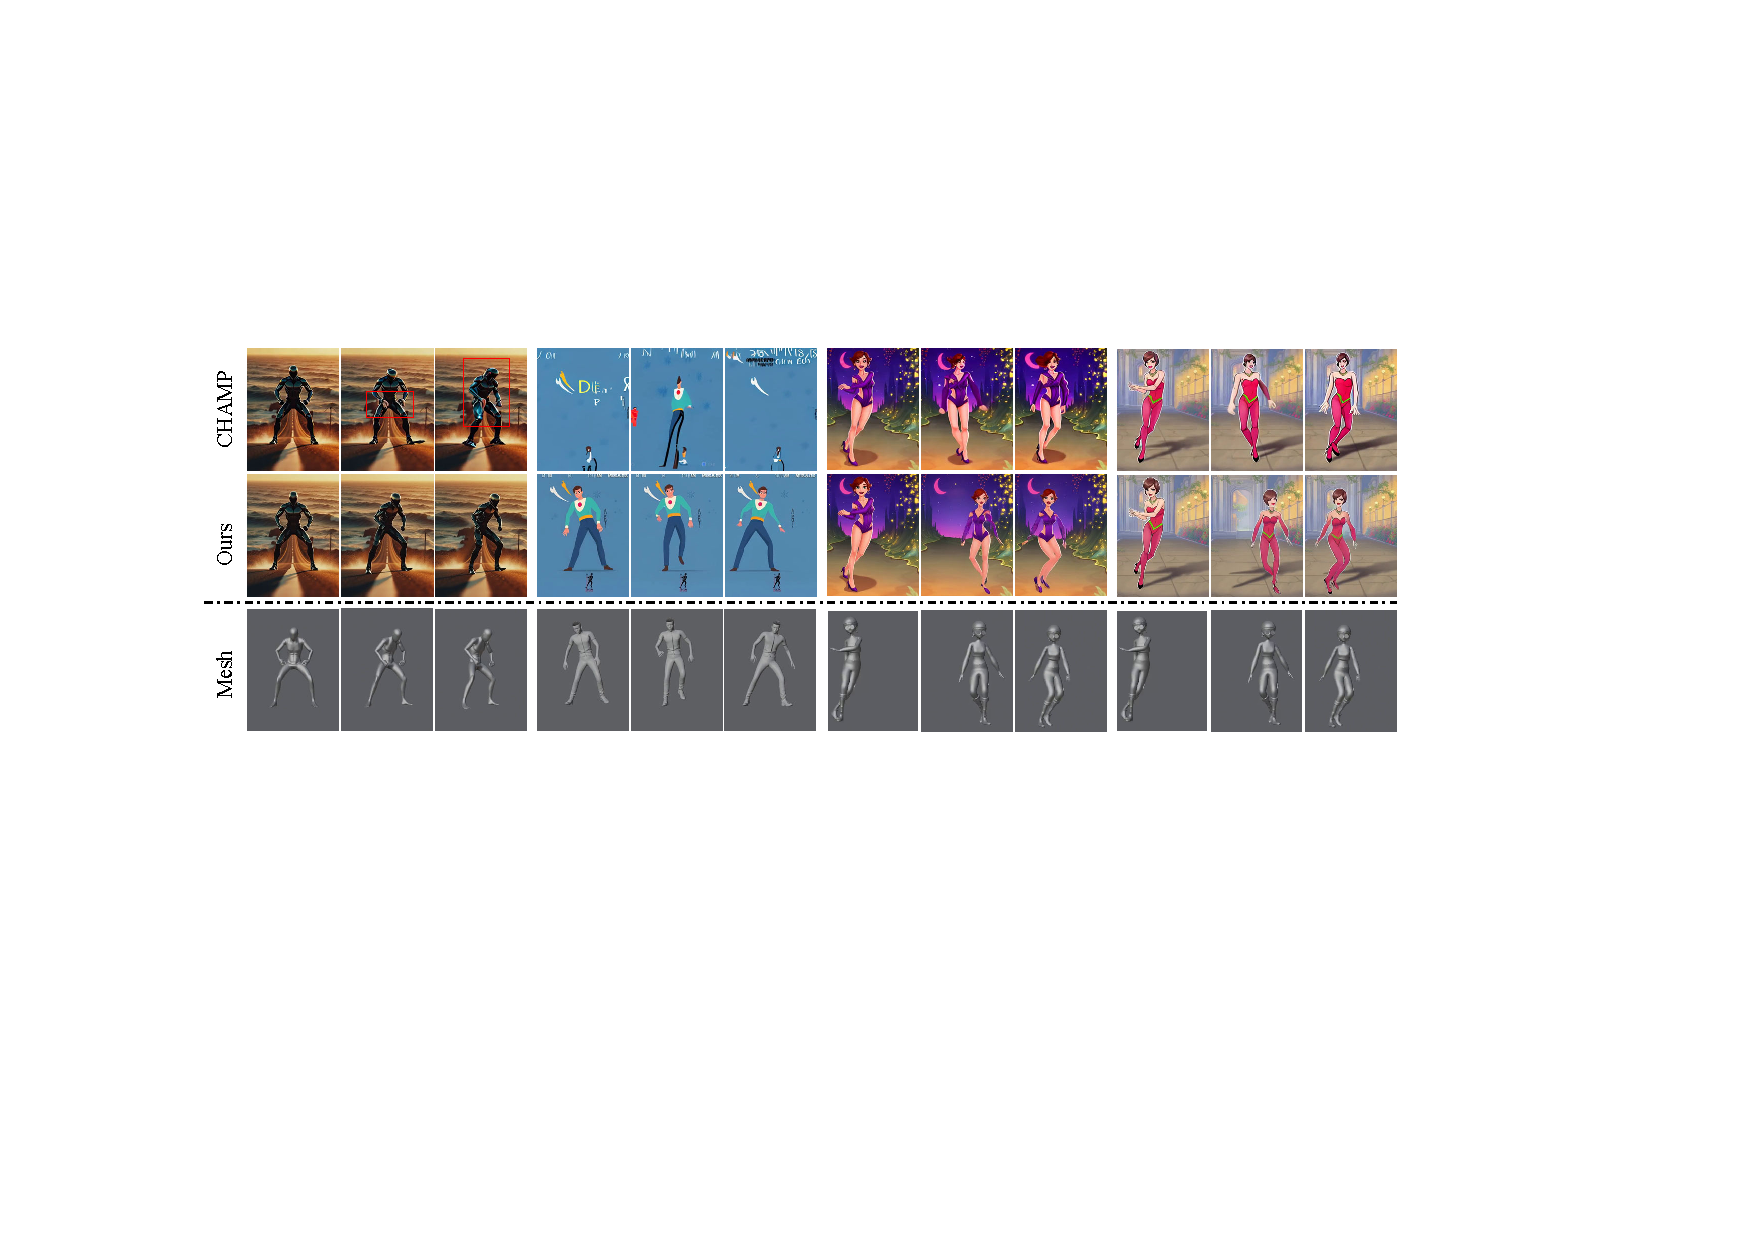
\includegraphics[width=0.97\textwidth]{pictures/m2v2.pdf}
    \caption{\textbf{Qualitative comparison on the animating mesh to video task} between our method and CHAMP~\cite{zhu2024champ}.}
    \label{fig:m2v2}
\end{figure*}

% \subsection{Physics-aware generation}
% \textbf{Qualitative results}. \ly{todo}.

% \begin{figure}
%     \centering
%     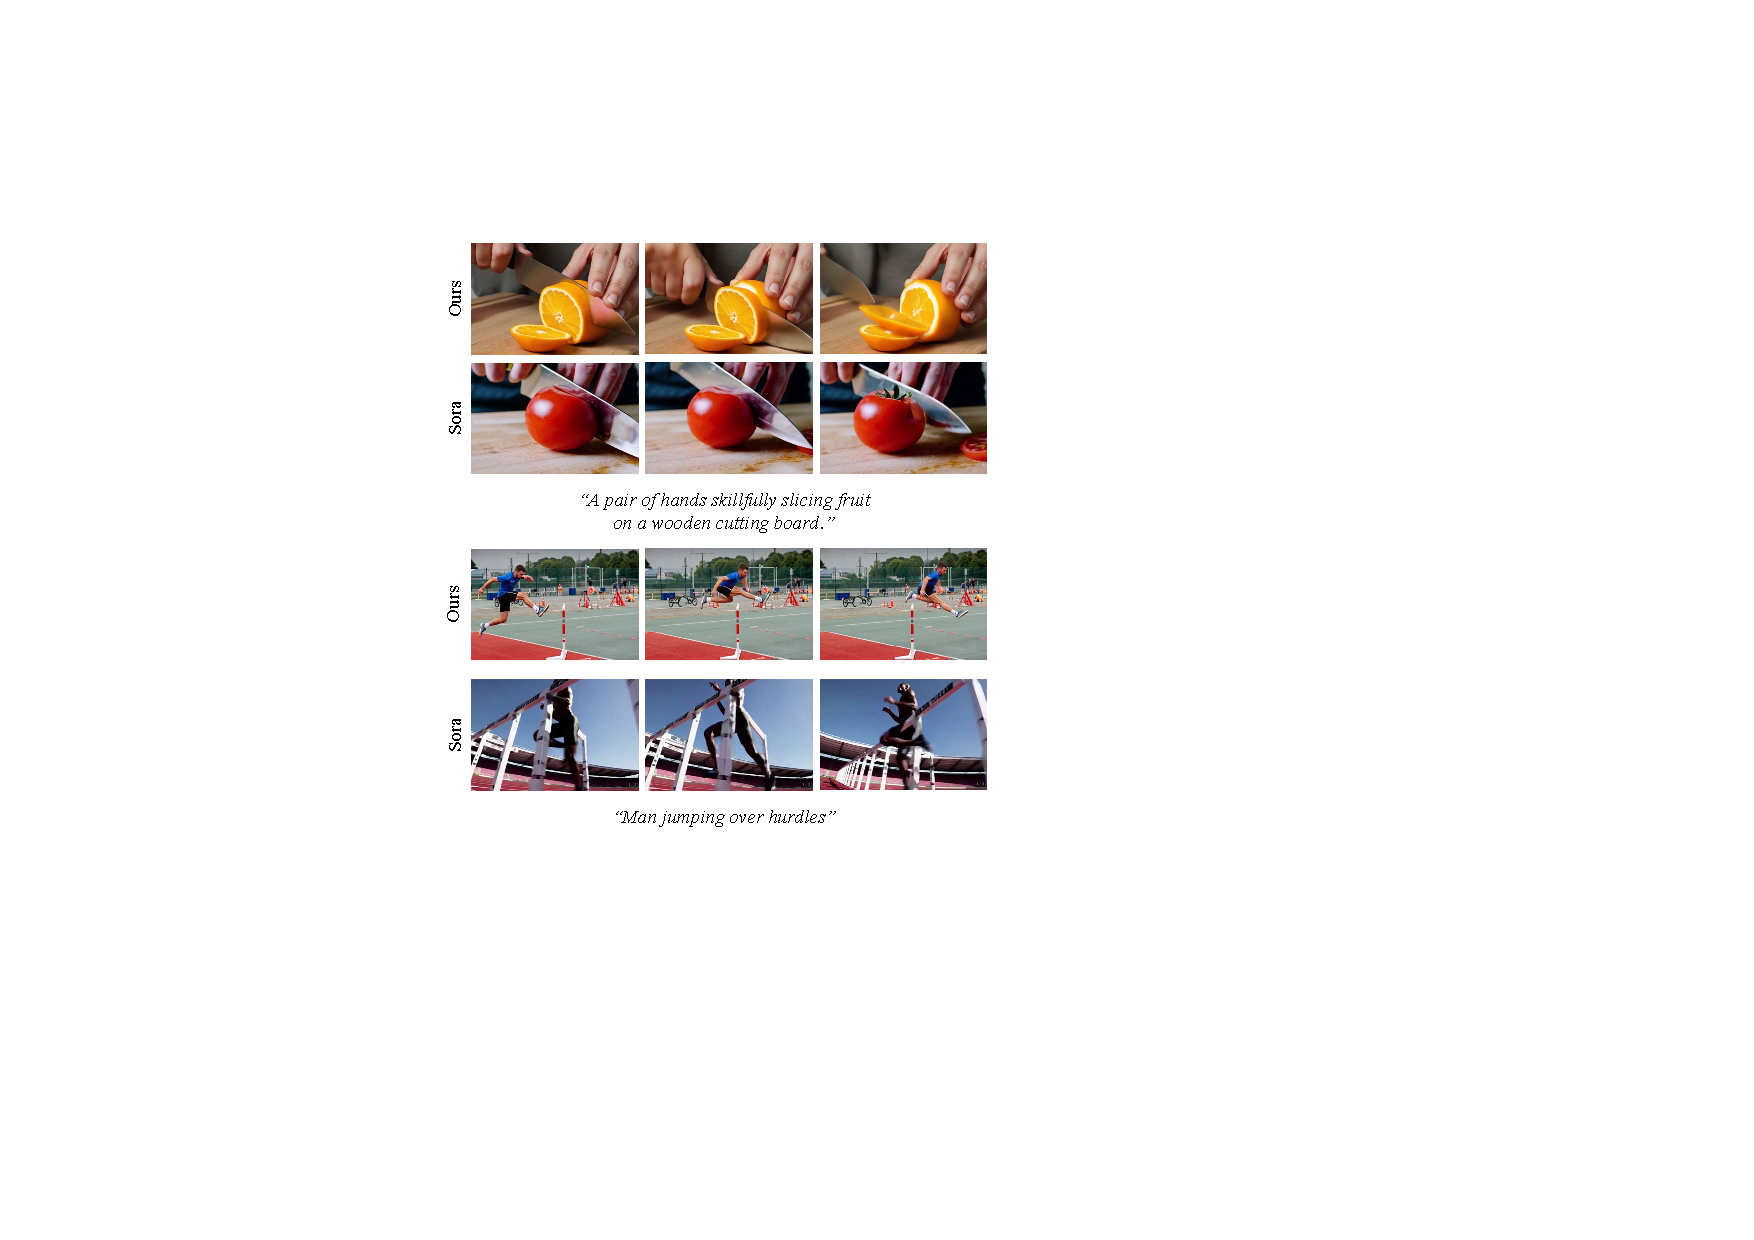
\includegraphics[width=\linewidth]{pictures/physic.pdf}
%     \caption{\ly{todo} \textbf{Results of physics-aware video generation.} I2V CogVideoX~\cite{yang2024cogvideox} model fails to generate physically plausible videos while our method utilizes the physics simulation to get a 3D tracking video for physics-aware video generation.}
%     \label{fig:physic}
% \end{figure}

\begin{figure*}
    \centering
    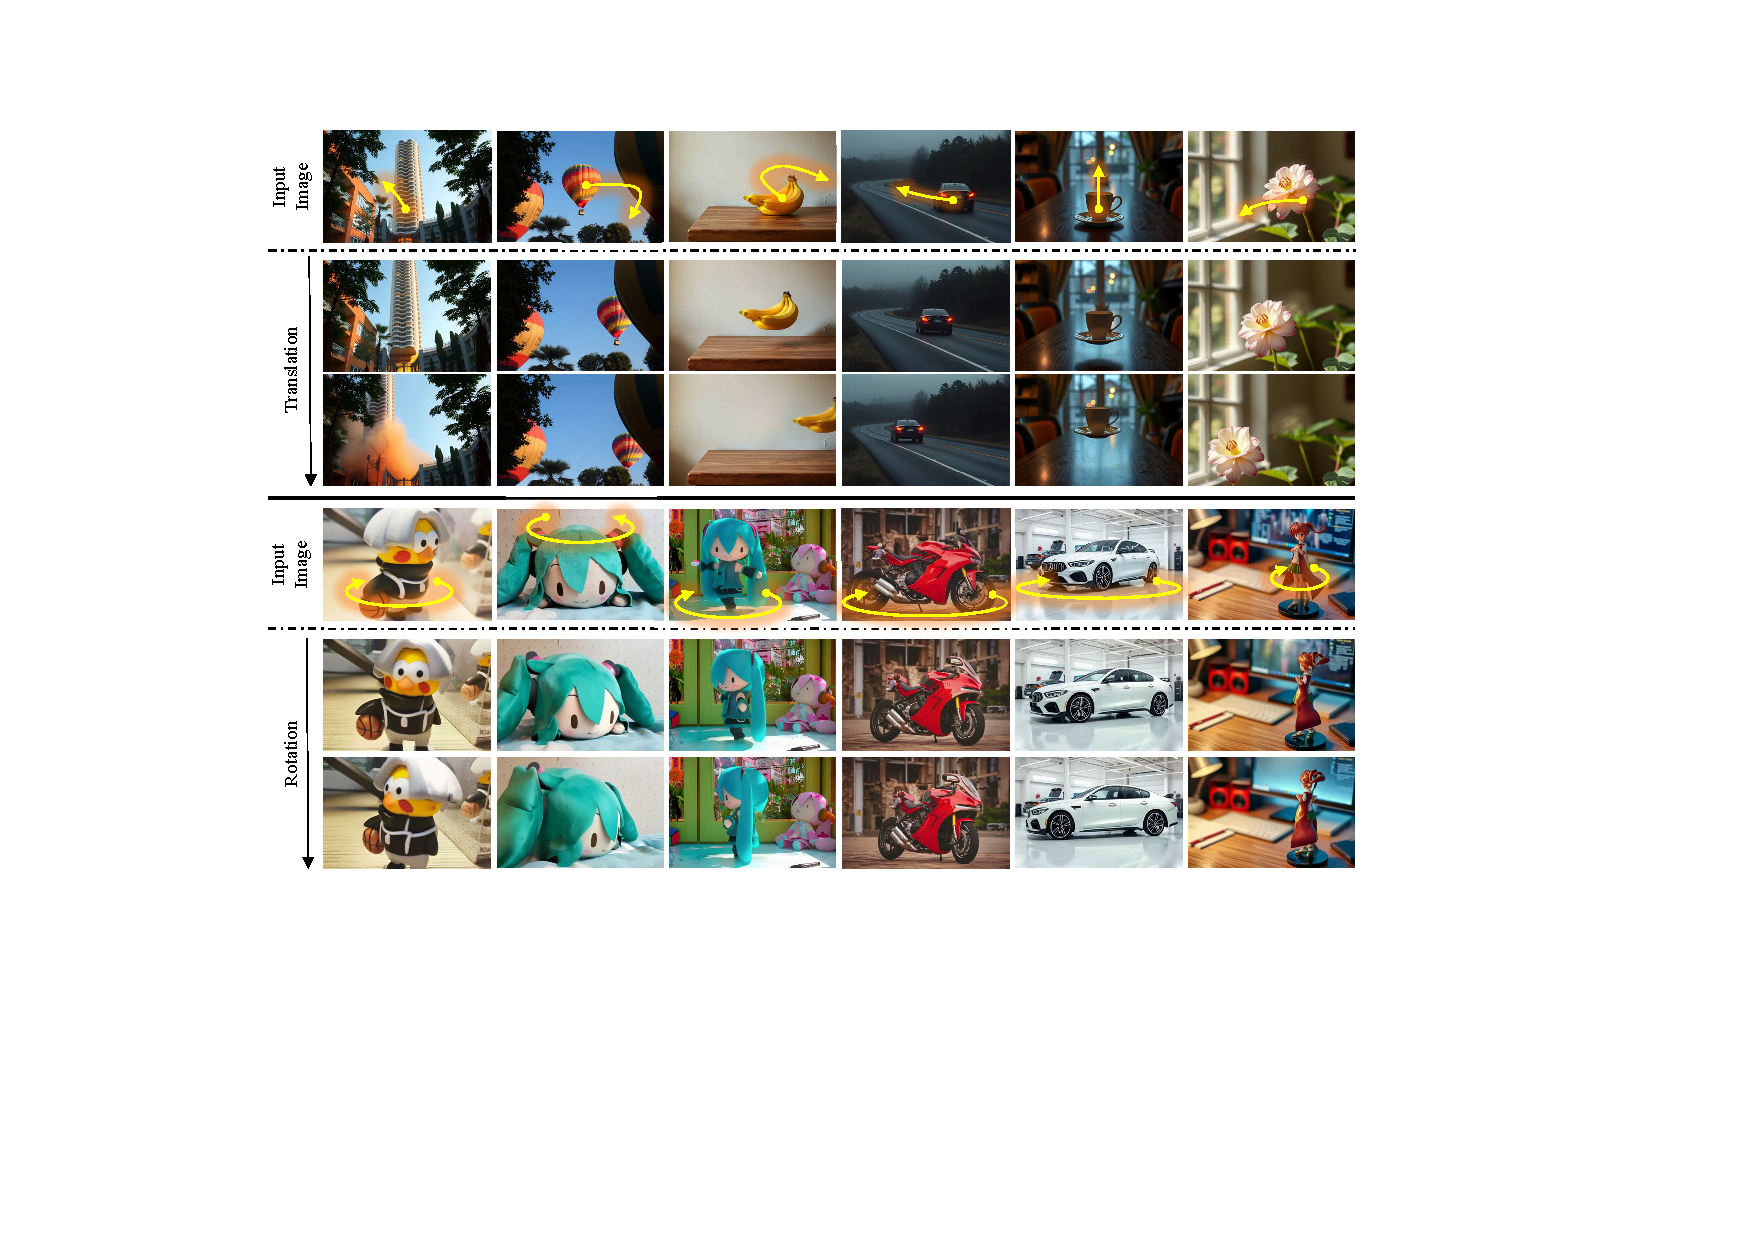
\includegraphics[width=\textwidth]{pictures/mani.pdf}
    \caption{\textbf{Qualitative results of our method on the object manipulation task}. The top part shows the results of translation while the bottom part shows the results of rotating the object.}
    \label{fig:mani2d}
\end{figure*}

\subsection{Object manipulation}
\textbf{Qualitative results}. For the object manipulation, we adopt the SAM~\cite{kirillov2023segment} and depth estimation models~\cite{bochkovskii2024depth,wang2024mogeunlockingaccuratemonocular} to get the object points. Then, we evaluate two kinds of manipulation, i.e. translation and rotation. The results are shown in Figure~\ref{fig:mani2d}, which demonstrate that \methodname achieves accurate object manipulation to produce photorealistic videos with strong multiview consistency for these objects.

\begin{table}[]
\setlength\tabcolsep{3pt}
\centering
\begin{tabular}{ccccccc}
\hline
Depth & Tracking    & \#Tracks & PSNR $\uparrow$ & SSIM $\uparrow$ & LPIPS $\downarrow$ & FVD $\downarrow$ \\ \hline
\checkmark &  & -      & 18.08           & 0.573           & 0.312              & 645.1            \\
& \checkmark  & 900    & 18.52           & 0.586           & 0.337              & 765.3            \\
& \checkmark  & 2500   & 19.17           & 0.632           & 0.263              & 566.4            \\
& \checkmark  & 4900   & \textbf{19.27}  & \textbf{0.658}  & \textbf{0.261}     & \textbf{551.3}   \\
& \checkmark  & 8100   & 19.11           & 0.649           & 0.262              & 599.0            \\ \hline
\end{tabular}
\caption{\textbf{Analysis of applying different 3D control signals for image to video generation}. We evaluate PSNR, SSIM, LPIPS, and FVD of generated videos on the validation set of the DAVIS and MiraData datasets. ``Depth'' means using depth maps as the 3D control signals. ``Tracking'' means using 3D tracking videos as the control signals. \#Tracks means the number of 3D  points used in the 3D tracking video.}
\vspace{-15pt}
\label{tab:ablation}
\end{table}

\subsection{Analysis}

We conduct analysis on the choice of 3D control signals, i.e. depth maps or 3D tracking videos, and the number of 3D tracking points.
To achieve this, we randomly selected 50 videos from the validation split of the DAVIS~\cite{Pont-Tuset_arXiv_2017} and MiraData~\cite{ju2024miradatalargescalevideodataset} video dataset. We extract the first-frame images as the input image and apply different models to re-generate these videos.
To evaluate the quality of the generated videos, we compute PSNR, SSIM~\cite{1284395}, LPIPS~\cite{zhang2018unreasonableeffectivenessdeepfeatures}, and FVD~\cite{unterthiner2019accurategenerativemodelsvideo} between the generated videos and the ground-truth videos.

\subsubsection{Depth maps vs. 3D tracking videos}

% Then, 3D tracking videos are extracted by SpatialTracker~\cite{xiao2024spatialtracker}. Then, we feed these inputs to our model to generate a video. 
To illustrate the effectiveness of our 3D tracking videos, we compare \methodname with a baseline using depth maps as conditions instead of 3D tracking videos. Specifically, the baseline adopts the same architecture as \methodname but replaces the 3D tracking video with a depth map video. We adopt the Depth Pro~\cite{bochkovskii2024depth} to generate the video depth video for this baseline method. As shown in \autoref{tab:ablation}, our model outperforms this baseline in all metrics, demonstrating that the 3D tracking videos provide a better signal for the diffusion model to recover groud-truth videos than the depth map conditions. \autoref{fig:depth-tracking} shows the generated videos, which demonstrate that our method produces more consistent videos with the ground truth. The main reason is that the 3D tracking videos effectively associate different frames of a video while the depth maps only provide some cues of the scene structures without constraining the motion of the video.

\begin{figure}
    \centering
    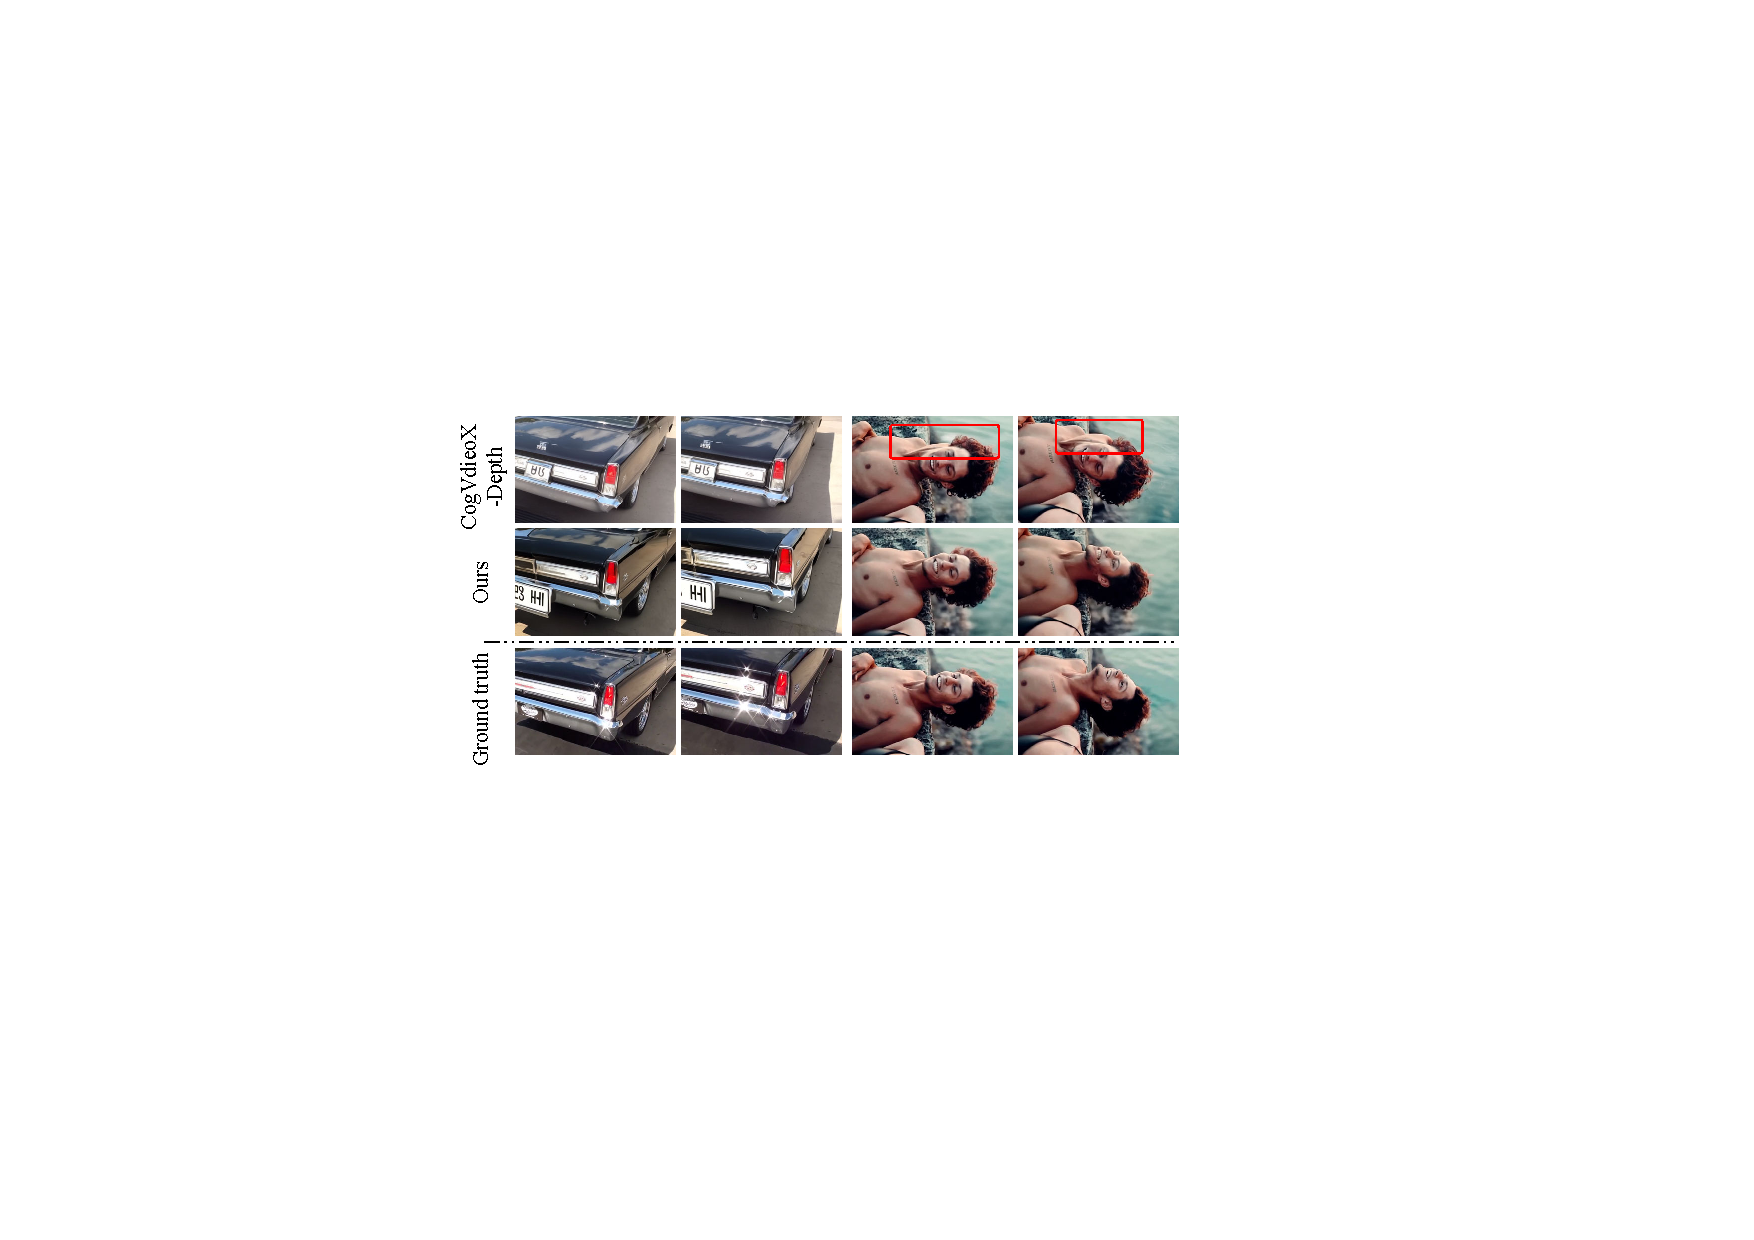
\includegraphics[width=\linewidth]{pictures/i2v1.pdf}
    \caption{\textbf{Generated videos using depth maps or 3D tracking videos as control signals.} Our 3D tracking videos provide better quality on the cross-frame consistency for video generation than depth maps.}
    \vspace{-15pt}
    \label{fig:depth-tracking}
\end{figure}

\subsubsection{Point density}

In \autoref{tab:ablation}, we further present an ablation study with varying numbers of 3D tracking points as control signals. The number of 3D tracking points ranges from 900 (30$\times$30) to 8100 (90$\times$90). Though the generated videos with 4900 tracking points perform slightly better than the other ones, the visual qualities of 2500, 4900, and 8100 tracking points are very similar to each other. Since tracking too many points with SpatialTracker~\cite{xiao2024spatialtracker} would be slow, we choose 4900 as our default setting in all our other experiments using 3D point tracking. 
% \ly{todo: add a figure of different tracking points (including tracking videos). in the supp}
% In the tracking videos, the size of the markers representing the 3D tracking points is determined based on the distance between two adjacent points, ensuring that the tracking video as an additional condition is not overly sparse. 
% We observe that the model performs best when the number of 3D tracking points is 4900. Before this point, the model's performance improves as the density of 3D tracking points increases. However, too dense 3D tracking points lead to a slightly decreased generation quality. The reason may be that the dense 3D tracking points are cluttered and some 3D points are not correctly tracked by the algorithm~\cite{xiao2024spatialtracker}.
% The reason is that as the density of 3D tracking points increases, the control area for each point decreases, weakening the representation of the overall structure of 3D objects in the video. This, in turn, impacts the effectiveness of the tracking video in representing 3D spatial structures.

% \textbf{Different tracking methods}. synthetic/SpatialTracker/Align3r

\subsubsection{Runtime}
In the inference stage, we employ the DDIM~\cite{song2020denoising} sampler with 50 steps, classifier-free guidance of magnitude 7.0, which costs about 2.5 minutes to generate 49 frames on a H800 GPU at a resolution of 480$\times$720.

\begin{figure}
    \centering
    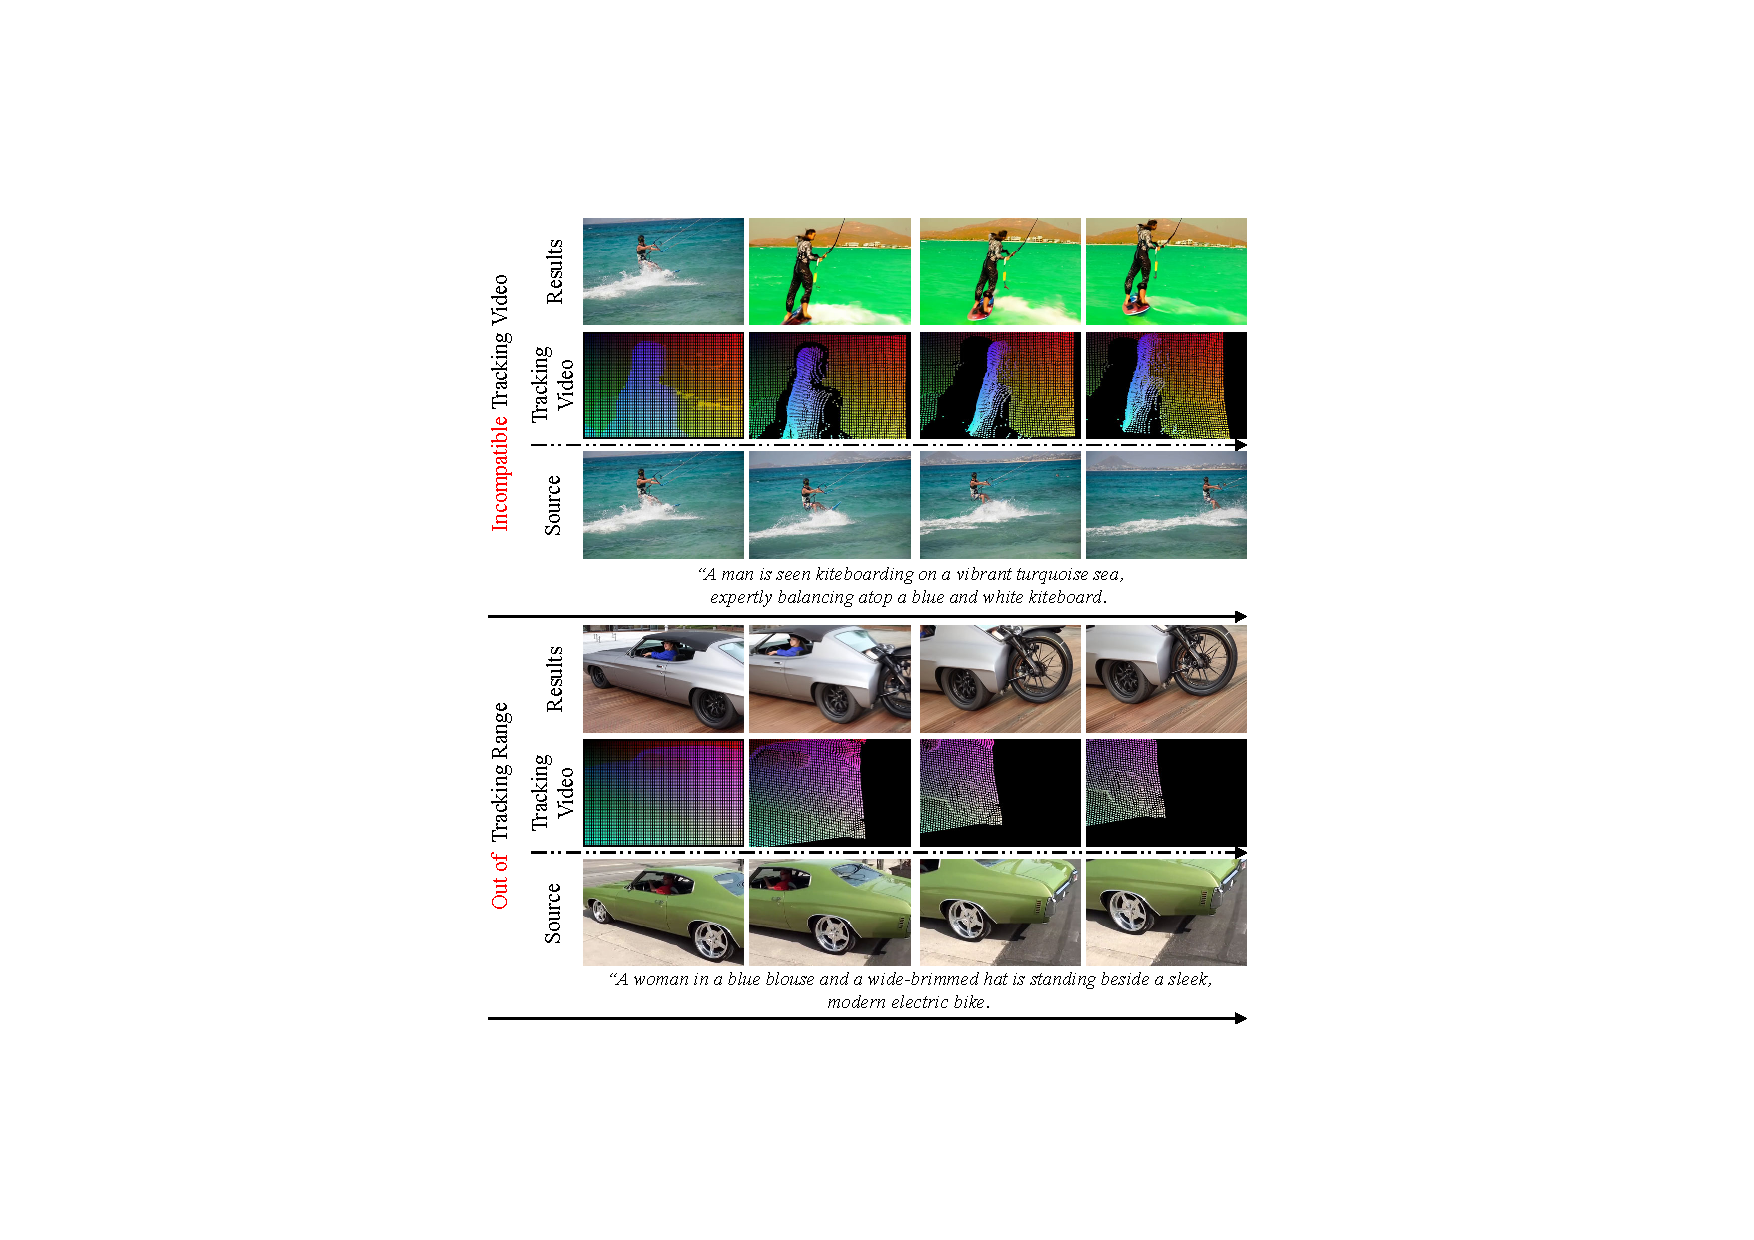
\includegraphics[width=\linewidth]{pictures/tracking.pdf}
    % \vspace{10pt}
    \caption{\textbf{Failure cases}. (Top) Incompatible tracking video. When a tracking video that does not correspond to the structures of the input image is provided, \methodname will generate a video with a scene transition to a compatible new scene.
    (Bottom) Out of tracking range. For regions without 3D tracking points, the tracking video fails to constrain these regions and \methodname may generate some uncontrolled content.} 
    \label{fig:tracking1}
\end{figure}